\documentclass{beamer}
\usepackage{ctex, hyperref}
\usepackage[T1]{fontenc}

% other packages
\usepackage{latexsym,amsmath,xcolor,multicol,booktabs,calligra}
\usepackage{graphicx,pstricks,listings,stackengine}

\title[LLMs in Economics]{\textbf{大语言模型在经济学中的应用}}
\subtitle{从API调用出发的学术应用实例}
\author{陆知雨}
\institute{中国财政发展协同创新中心\\
\vspace{2mm}财政学基地班22}
\date{\today}
\usetheme[hideothersubsections]{Hannover}

% defs
\def\cmd#1{\texttt{\color{red}\footnotesize $\backslash$#1}}
\def\env#1{\texttt{\color{blue}\footnotesize #1}}
\definecolor{deepblue}{rgb}{0,0,0.5}
\definecolor{deepred}{rgb}{0.6,0,0}
\definecolor{deepgreen}{rgb}{0,0.5,0}
\definecolor{halfgray}{gray}{0.55}


\definecolor{dkgreen}{rgb}{0,0.6,0}
\definecolor{gray}{rgb}{0.5,0.5,0.5}
\definecolor{mauve}{rgb}{0.58,0,0.82}
\lstset{frame=tb,
  language=Python,
  aboveskip=1mm,
  belowskip=1mm,
  showstringspaces=false,
  columns=flexible,
  basicstyle={\scriptsize\ttfamily},
  numbers=none,
  numberstyle=\scriptsize\color{gray},
  keywordstyle=\color{blue},
  commentstyle=\color{dkgreen},
  stringstyle=\color{mauve},
  breaklines=true,
  breakatwhitespace=true,
  tabsize=2
}
\AtBeginSection[]{
	\begin{frame}
		\tableofcontents[currentsection]
	\end{frame}
} % 每到新的一节(Section)显示大纲

\begin{document}

% TITLE PAGE
\begin{frame}
  \titlepage
\end{frame}

% TABLE OF CONTENTS
\begin{frame}{目录}
    \tableofcontents[hideallsubsections]
\end{frame}

%=================================================
\section{引言}
%=================================================
\begin{frame}{引言}
  \begin{itemize}
    \item \textbf{文本是知识的载体} 
    \item 合理处理文本,是构造解释、被解释变量的关键
    \item 当前处理文本数据以文本\textbf{匹配}为核心:
  \begin{enumerate}
  	\item 使用正则表达式提取CEO简历数据
	\item 使用情感词词典判断媒体情绪
	\item 使用数字化转型词典判断企业是否发生数字化转型
\end{enumerate}
    \item 在面临更加“复杂”的文本环境时,由于难以穷尽各类匹配情况,研究者需要手动操作进行提取。
    \item \textbf{但是,机器可以替代重复简单劳动!}
  \end{itemize}
\end{frame}

\begin{frame}[fragile]{示例1}
  \begin{itemize}
    \item 如何判断普通网民的情绪?
    \item \textbf{与媒体情绪的区别:} 网络留言更为随意,文本样式多变
    \item \textbf{例如(摘自东方财富股吧):}
  \begin{enumerate}
	\item 工行没吃饭呢林黛玉似的好柔弱
	\item 顶王粉丝光荣站岗
\end{enumerate}
  \end{itemize}
  \pause
    \begin{figure}[htpb]
  	\centering
  	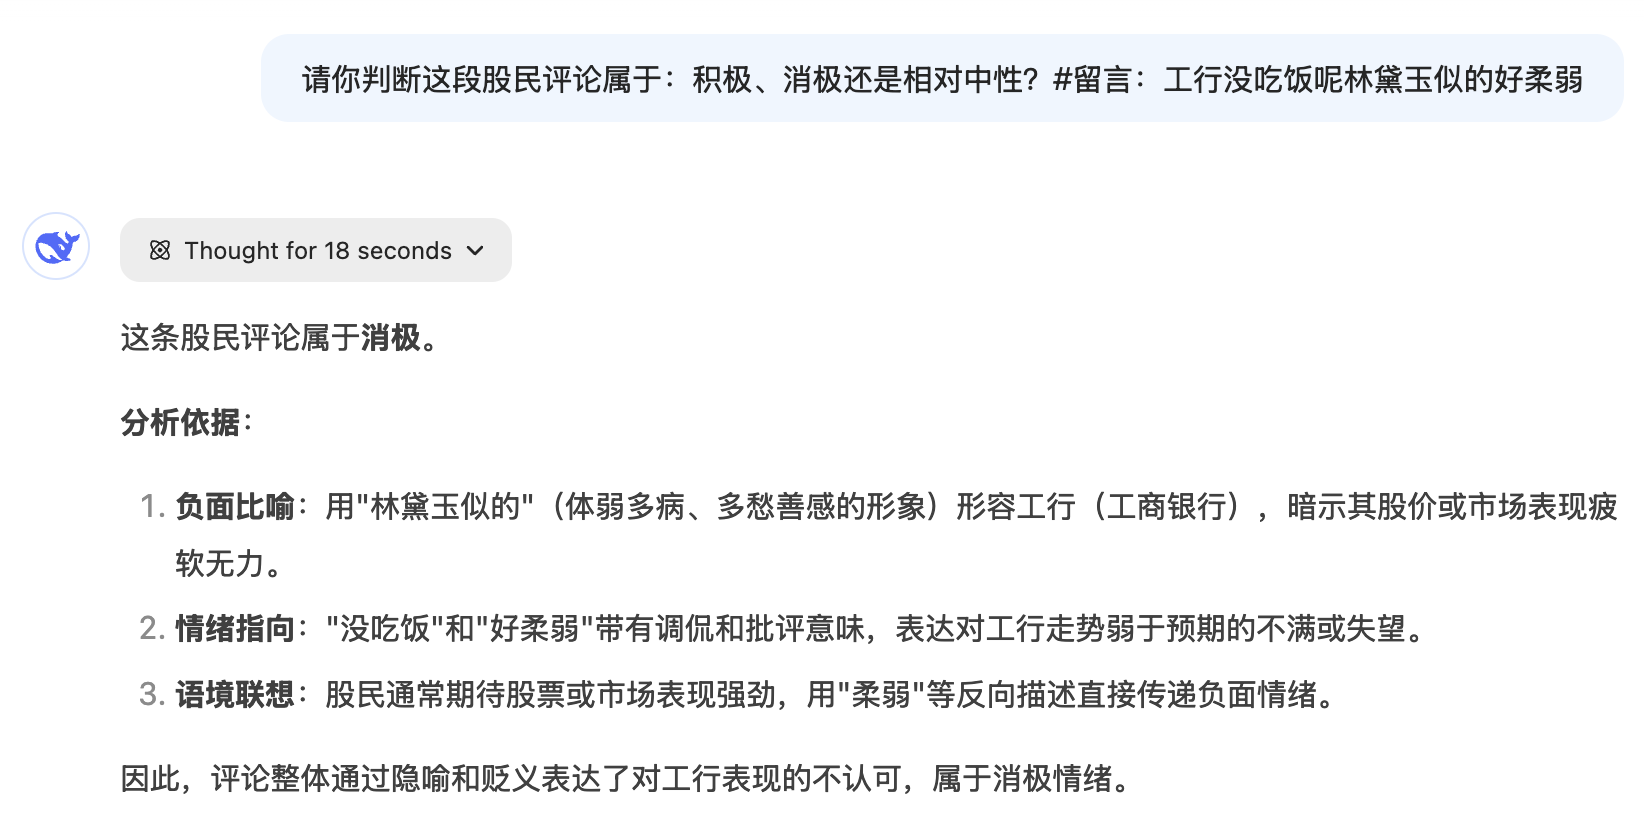
\includegraphics[width=0.9\linewidth]{figs/林黛玉.png}
  \end{figure}
\end{frame}
\begin{frame}[fragile]{示例1}
	\begin{itemize}
		\item\textbf{ 如何判断普通网民的情绪?}
		\item \textbf{与媒体文本的区别:} 网络留言更为随意,文本样式多变
		\item \textbf{例如(摘自东方财富股吧):}
		\begin{enumerate}
			\item 工行没吃饭呢林黛玉似的好柔弱
			\item 顶王粉丝光荣站岗
		\end{enumerate}
	\end{itemize}
	\begin{figure}[htpb]
		\centering
		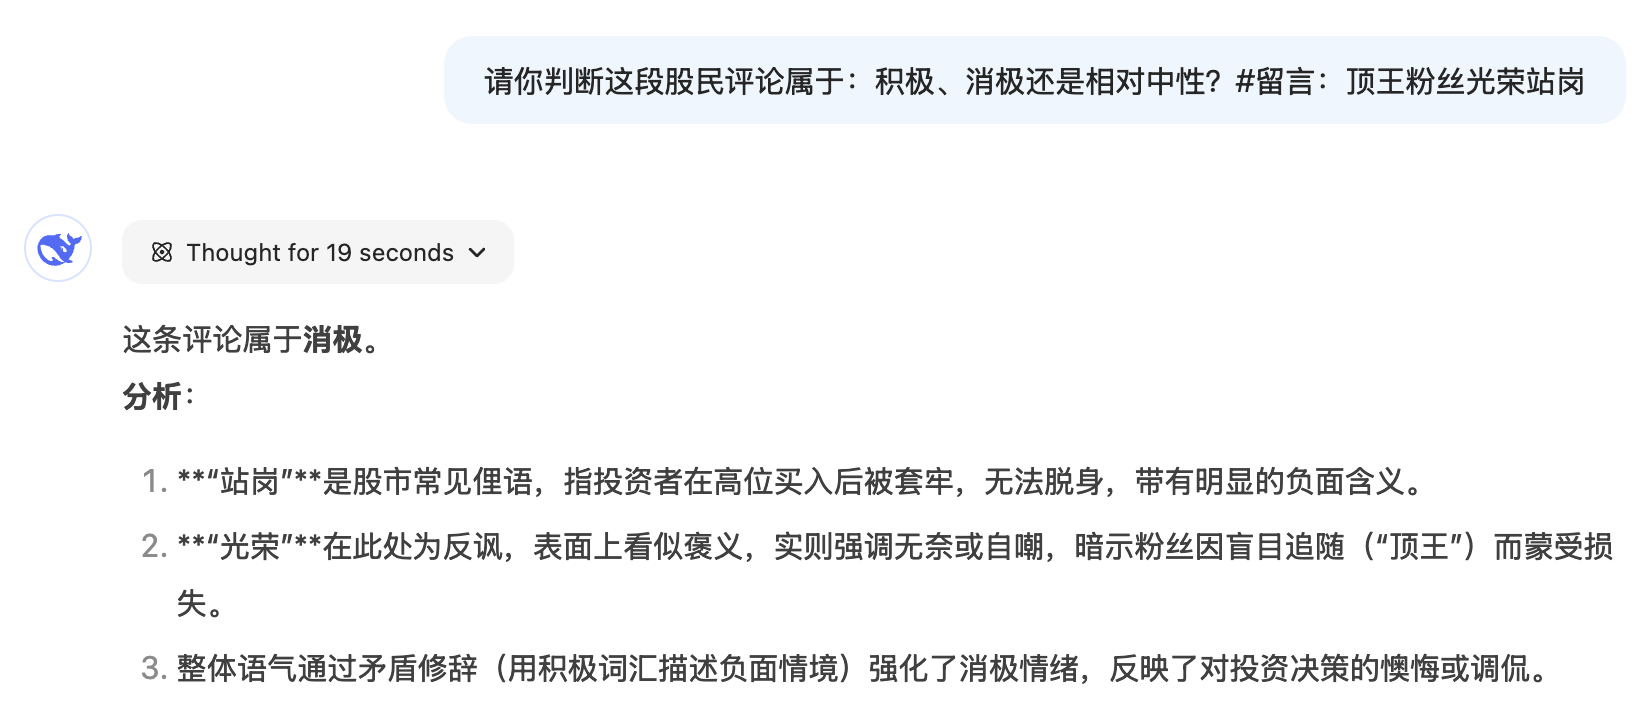
\includegraphics[width=0.9\linewidth]{figs/顶王.png}
	\end{figure}
\end{frame}

\begin{frame}{示例2}
	\begin{itemize}
	\item \textbf{如何提取文本中的关键信息?}
	\item \textbf{当目标文本格式不统一,正则表达式提取就变得极为复杂} 
	\item \textbf{例如:}从政府工作报告提取经济增长目标值
\end{itemize}
    \begin{columns}
	\begin{column}{.5\textwidth}
		\begin{itemize}
		\item 使用正则表达式流程:
		\begin{enumerate}
			\item 读取多篇文献,找到几类常见用语,并转译成正则表达式
			\item 使用正则表达式进行匹配
			\item 匹配后检查未匹配到的城市的文本,完善正则表达式,返回步骤2
		\end{enumerate} 
	\end{itemize}
	\end{column}
	\begin{column}{.45\textwidth}
			\begin{itemize}
			\item 使用大语言模型:
		\end{itemize}
	\begin{figure}[htpb]
	\centering
	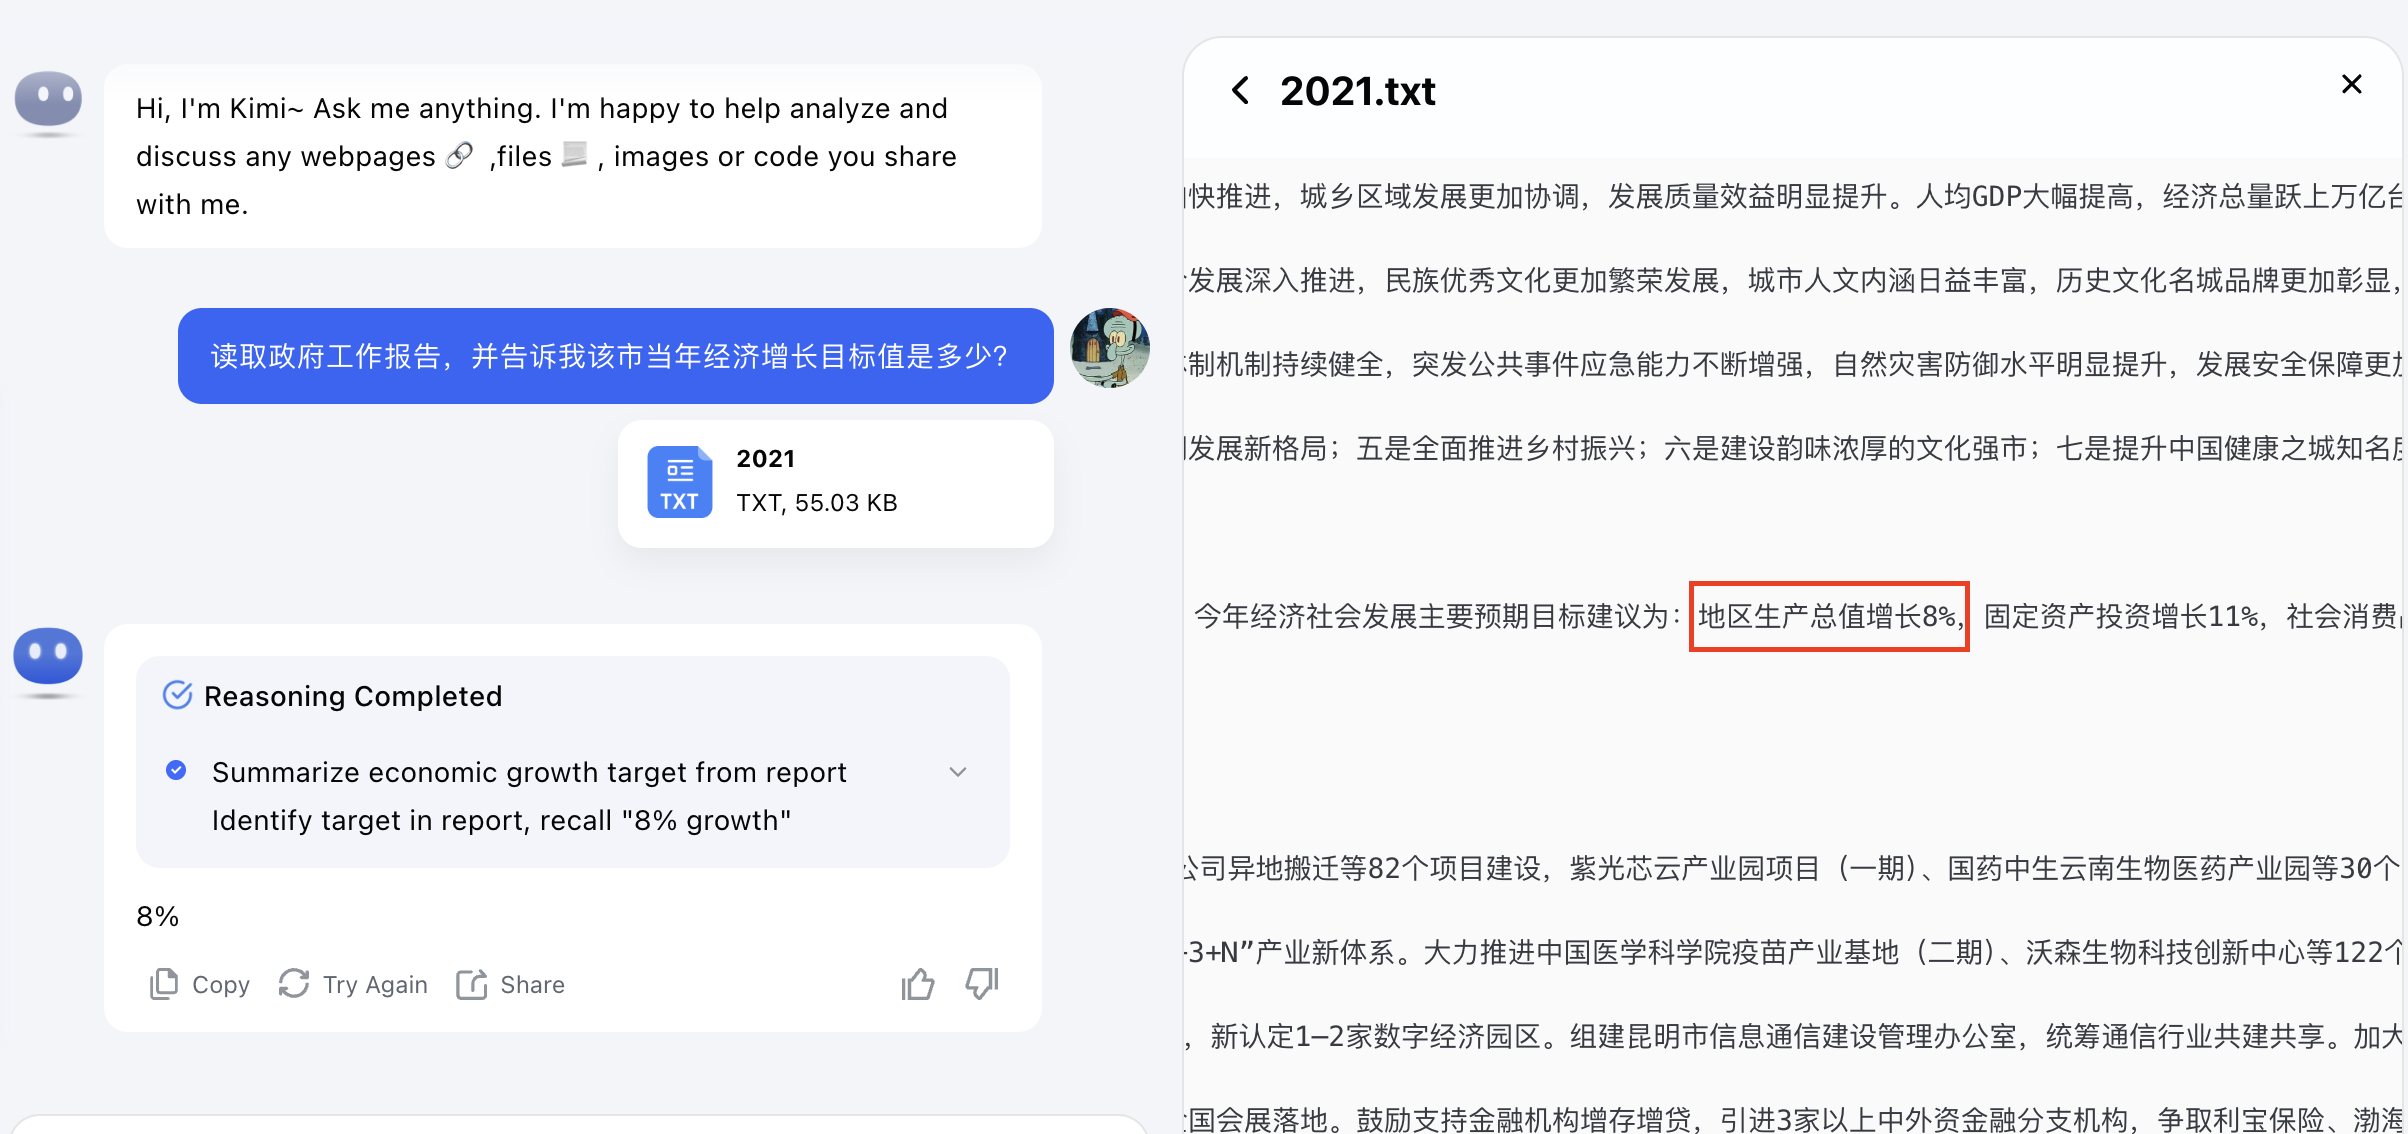
\includegraphics[width=1.34\linewidth]{figs/经济增长.png}
\end{figure}
	\end{column}
\end{columns}
\end{frame}
%=================================================
\section{大语言模型的代码调用}
%=================================================
\begin{frame}{代码调用与网页调用对比}
    \begin{itemize}
        \item 但是,如果待处理样本量过大,从网页逐个处理是否反而繁琐?
        \item \textbf{机器可以替代重复简单劳动!}
        \pause 
        \item 实际上,除了相对易用的网页端口,厂商还提供了API(编程接口),供开发者在代码中嵌入大语言模型。这为批量处理文本提供条件。
      \end{itemize}
    \begin{columns}
	\begin{column}{.5\textwidth}
		\begin{figure}[htpb]
		\centering
		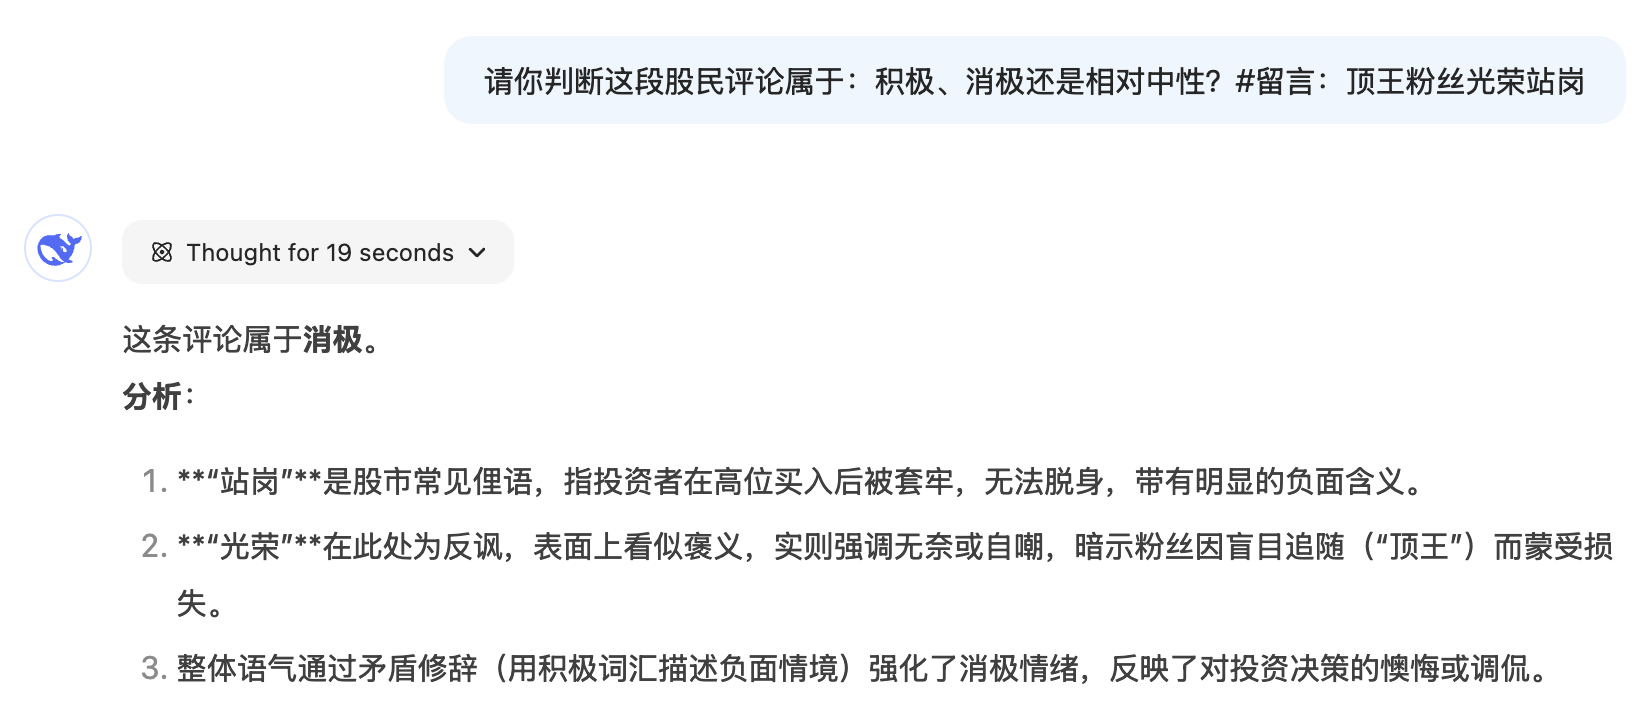
\includegraphics[width=1\linewidth]{figs/顶王.png}
	\end{figure}
	\end{column}
	
	\begin{column}{.5\textwidth}
		\begin{figure}[htpb]
			\centering
			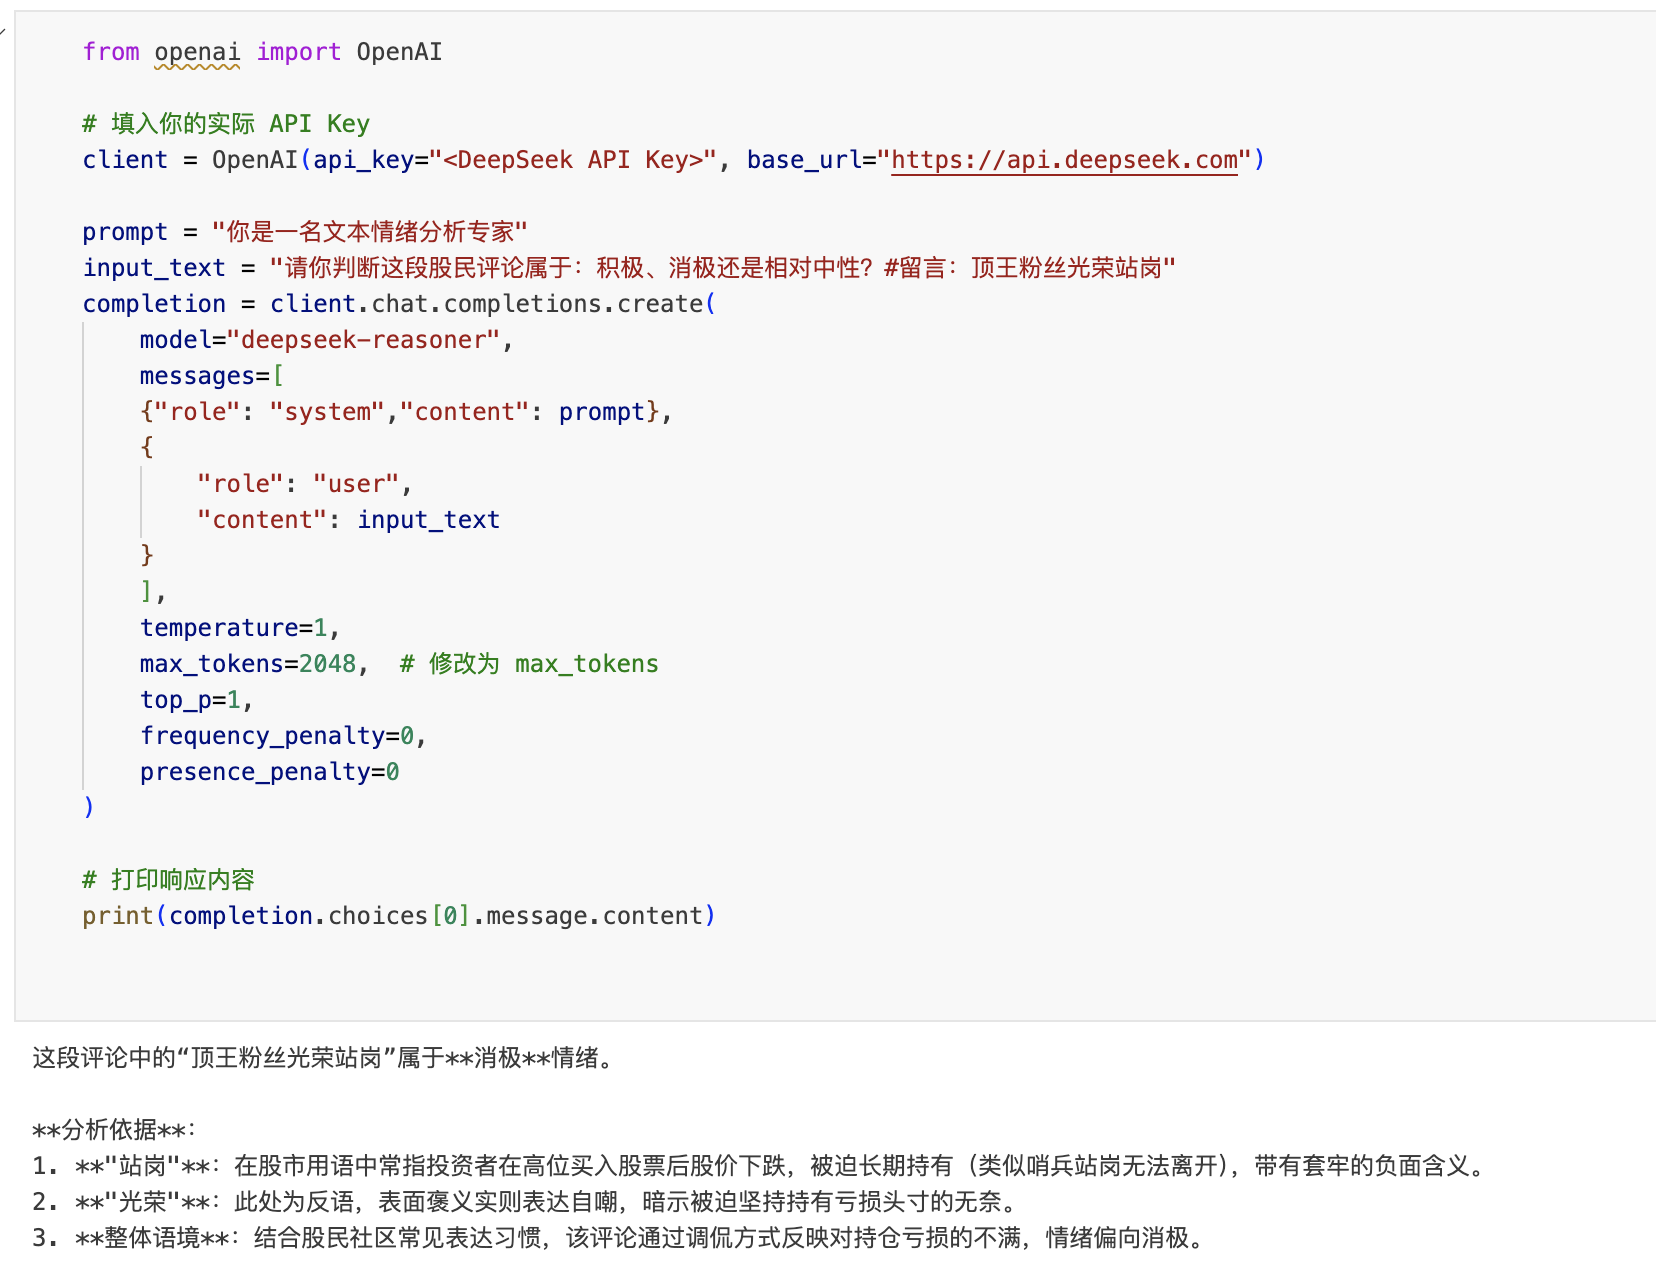
\includegraphics[width=1\linewidth]{figs/顶王2.png}
		\end{figure}
	\end{column}
\end{columns}

  
\end{frame}

\begin{frame}{主流大语言模型API Key的获取}
    \begin{itemize}
        \item  \textbf{国内厂商:}一般而言,国内厂商的API平台与大语言模型平台在相邻页面。以deepseek为例
        	\begin{figure}[htpb]
        	\centering
        	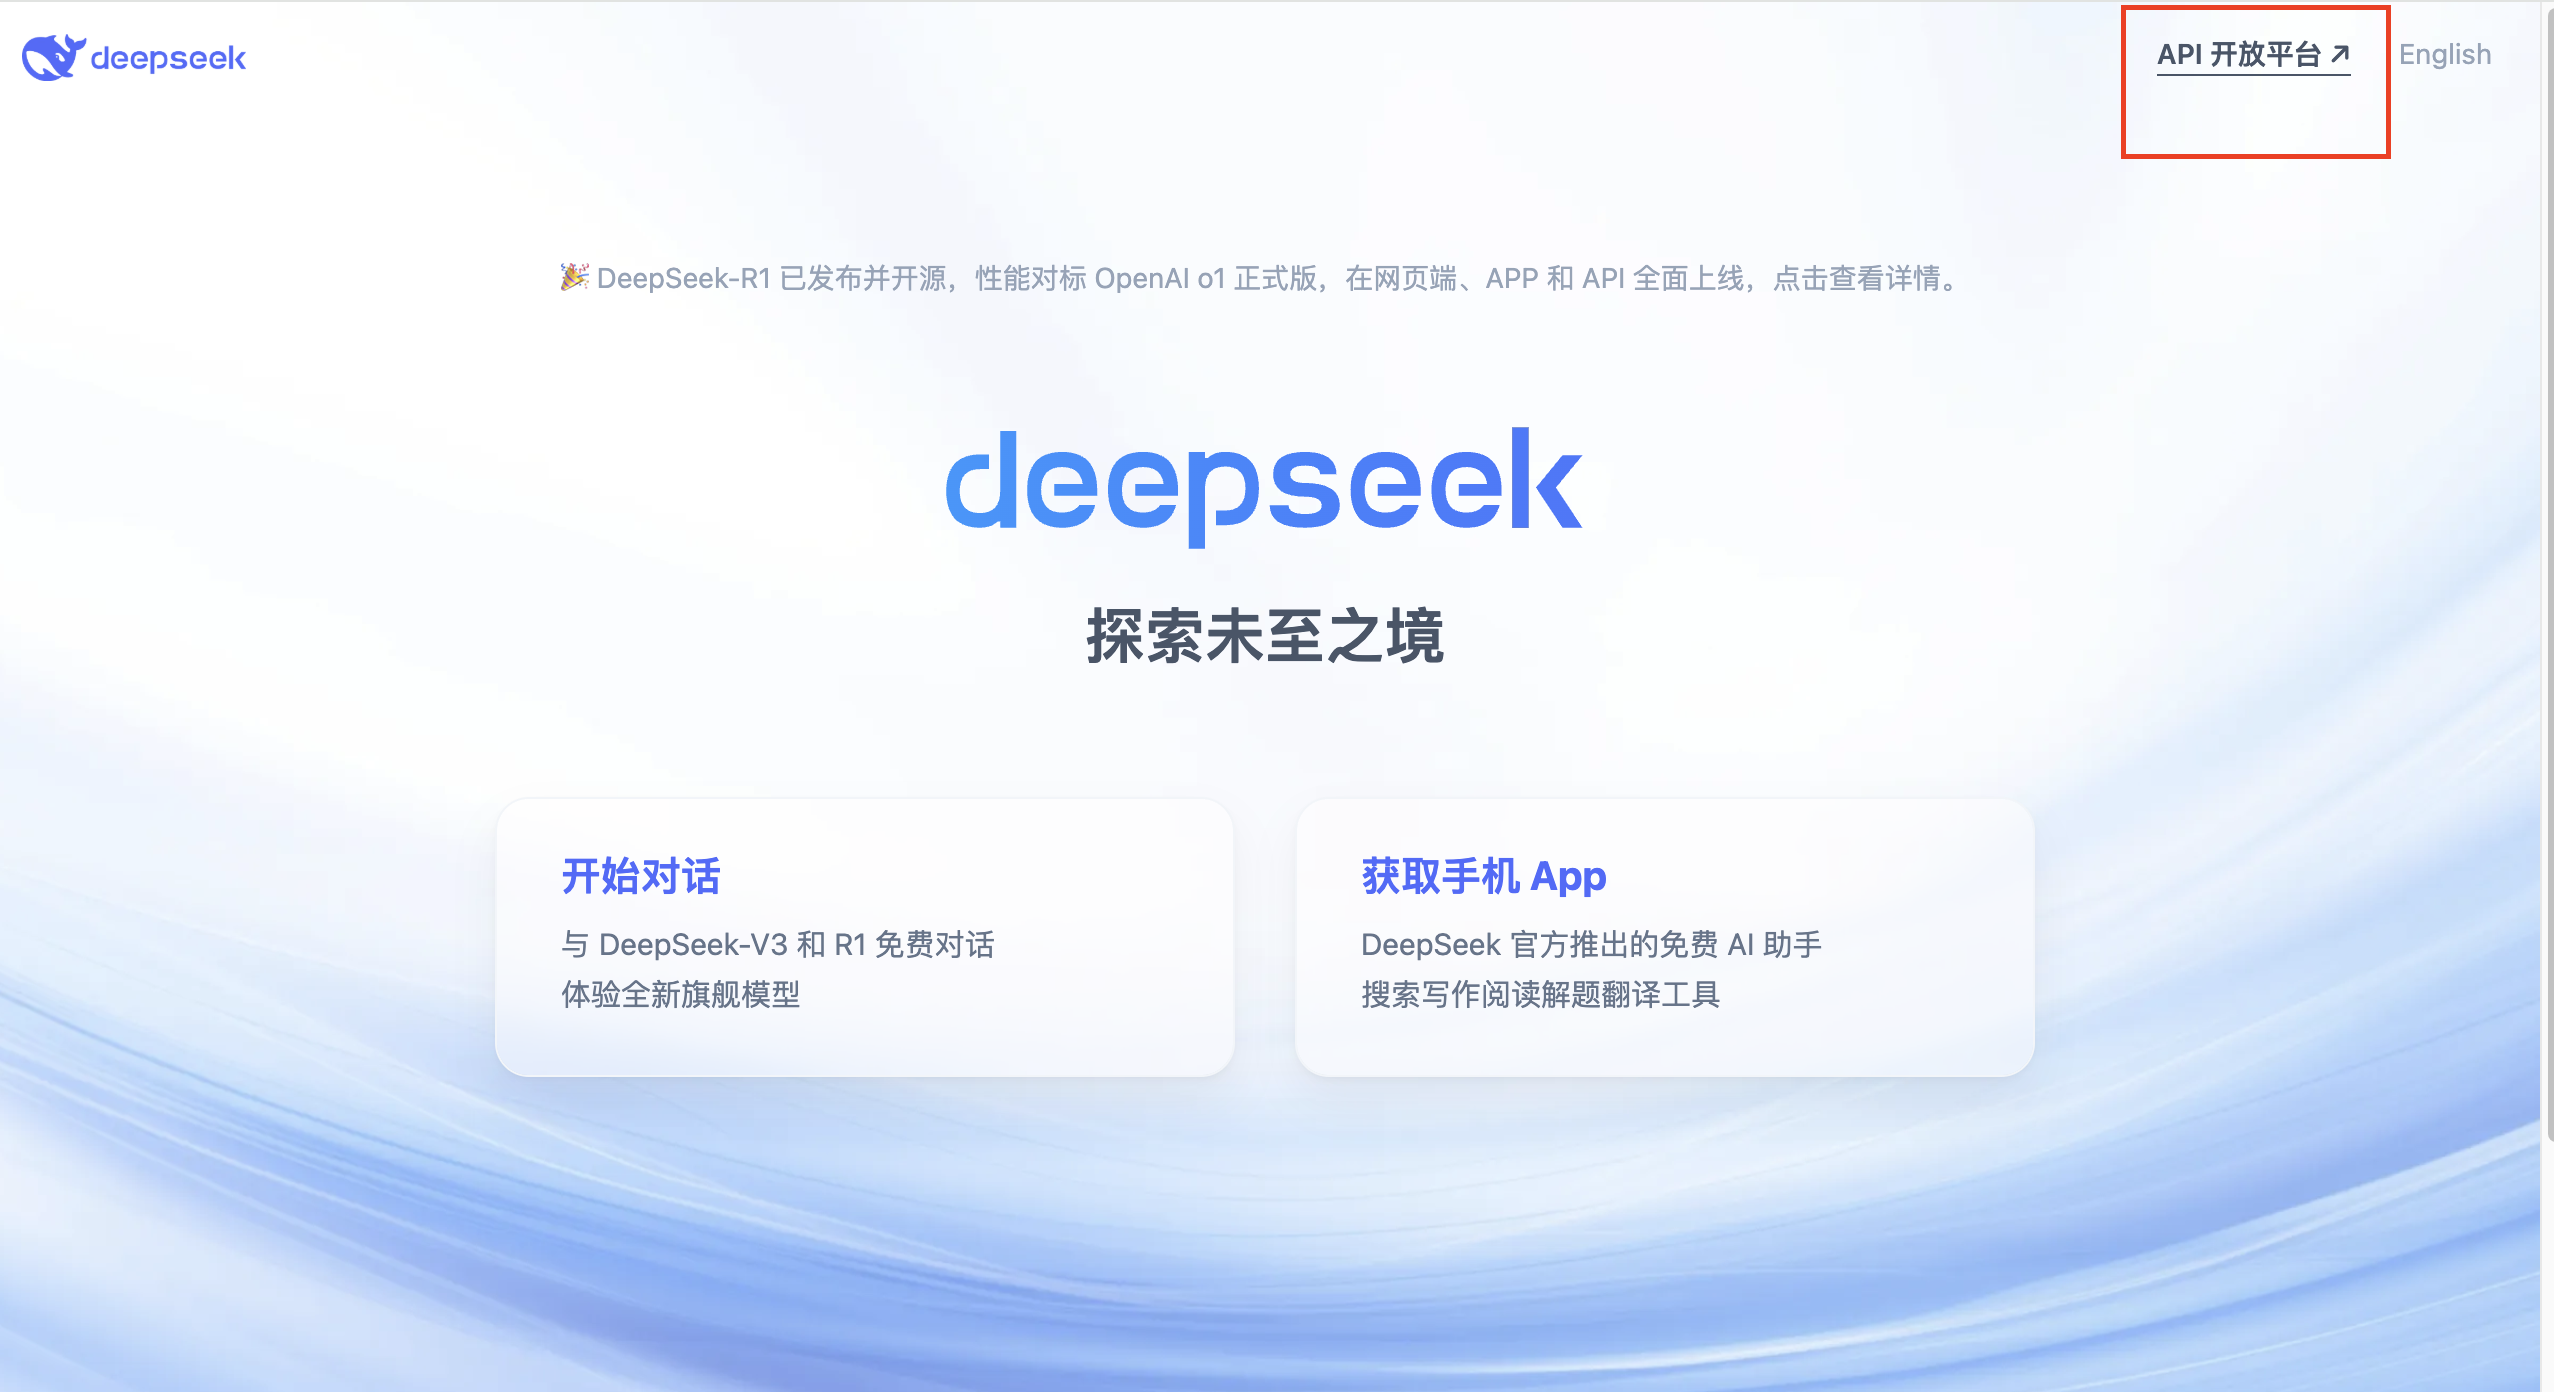
\includegraphics[width=1\linewidth]{figs/API1.png}
        \end{figure}
   
      \end{itemize}
\end{frame}
\begin{frame}{主流大语言模型API Key的获取}
	\begin{itemize}
		\item  \textbf{国内厂商:}一般而言,国内厂商的API平台与大语言模型平台在相邻页面。以deepseek为例
		\begin{figure}[htpb]
			\centering
			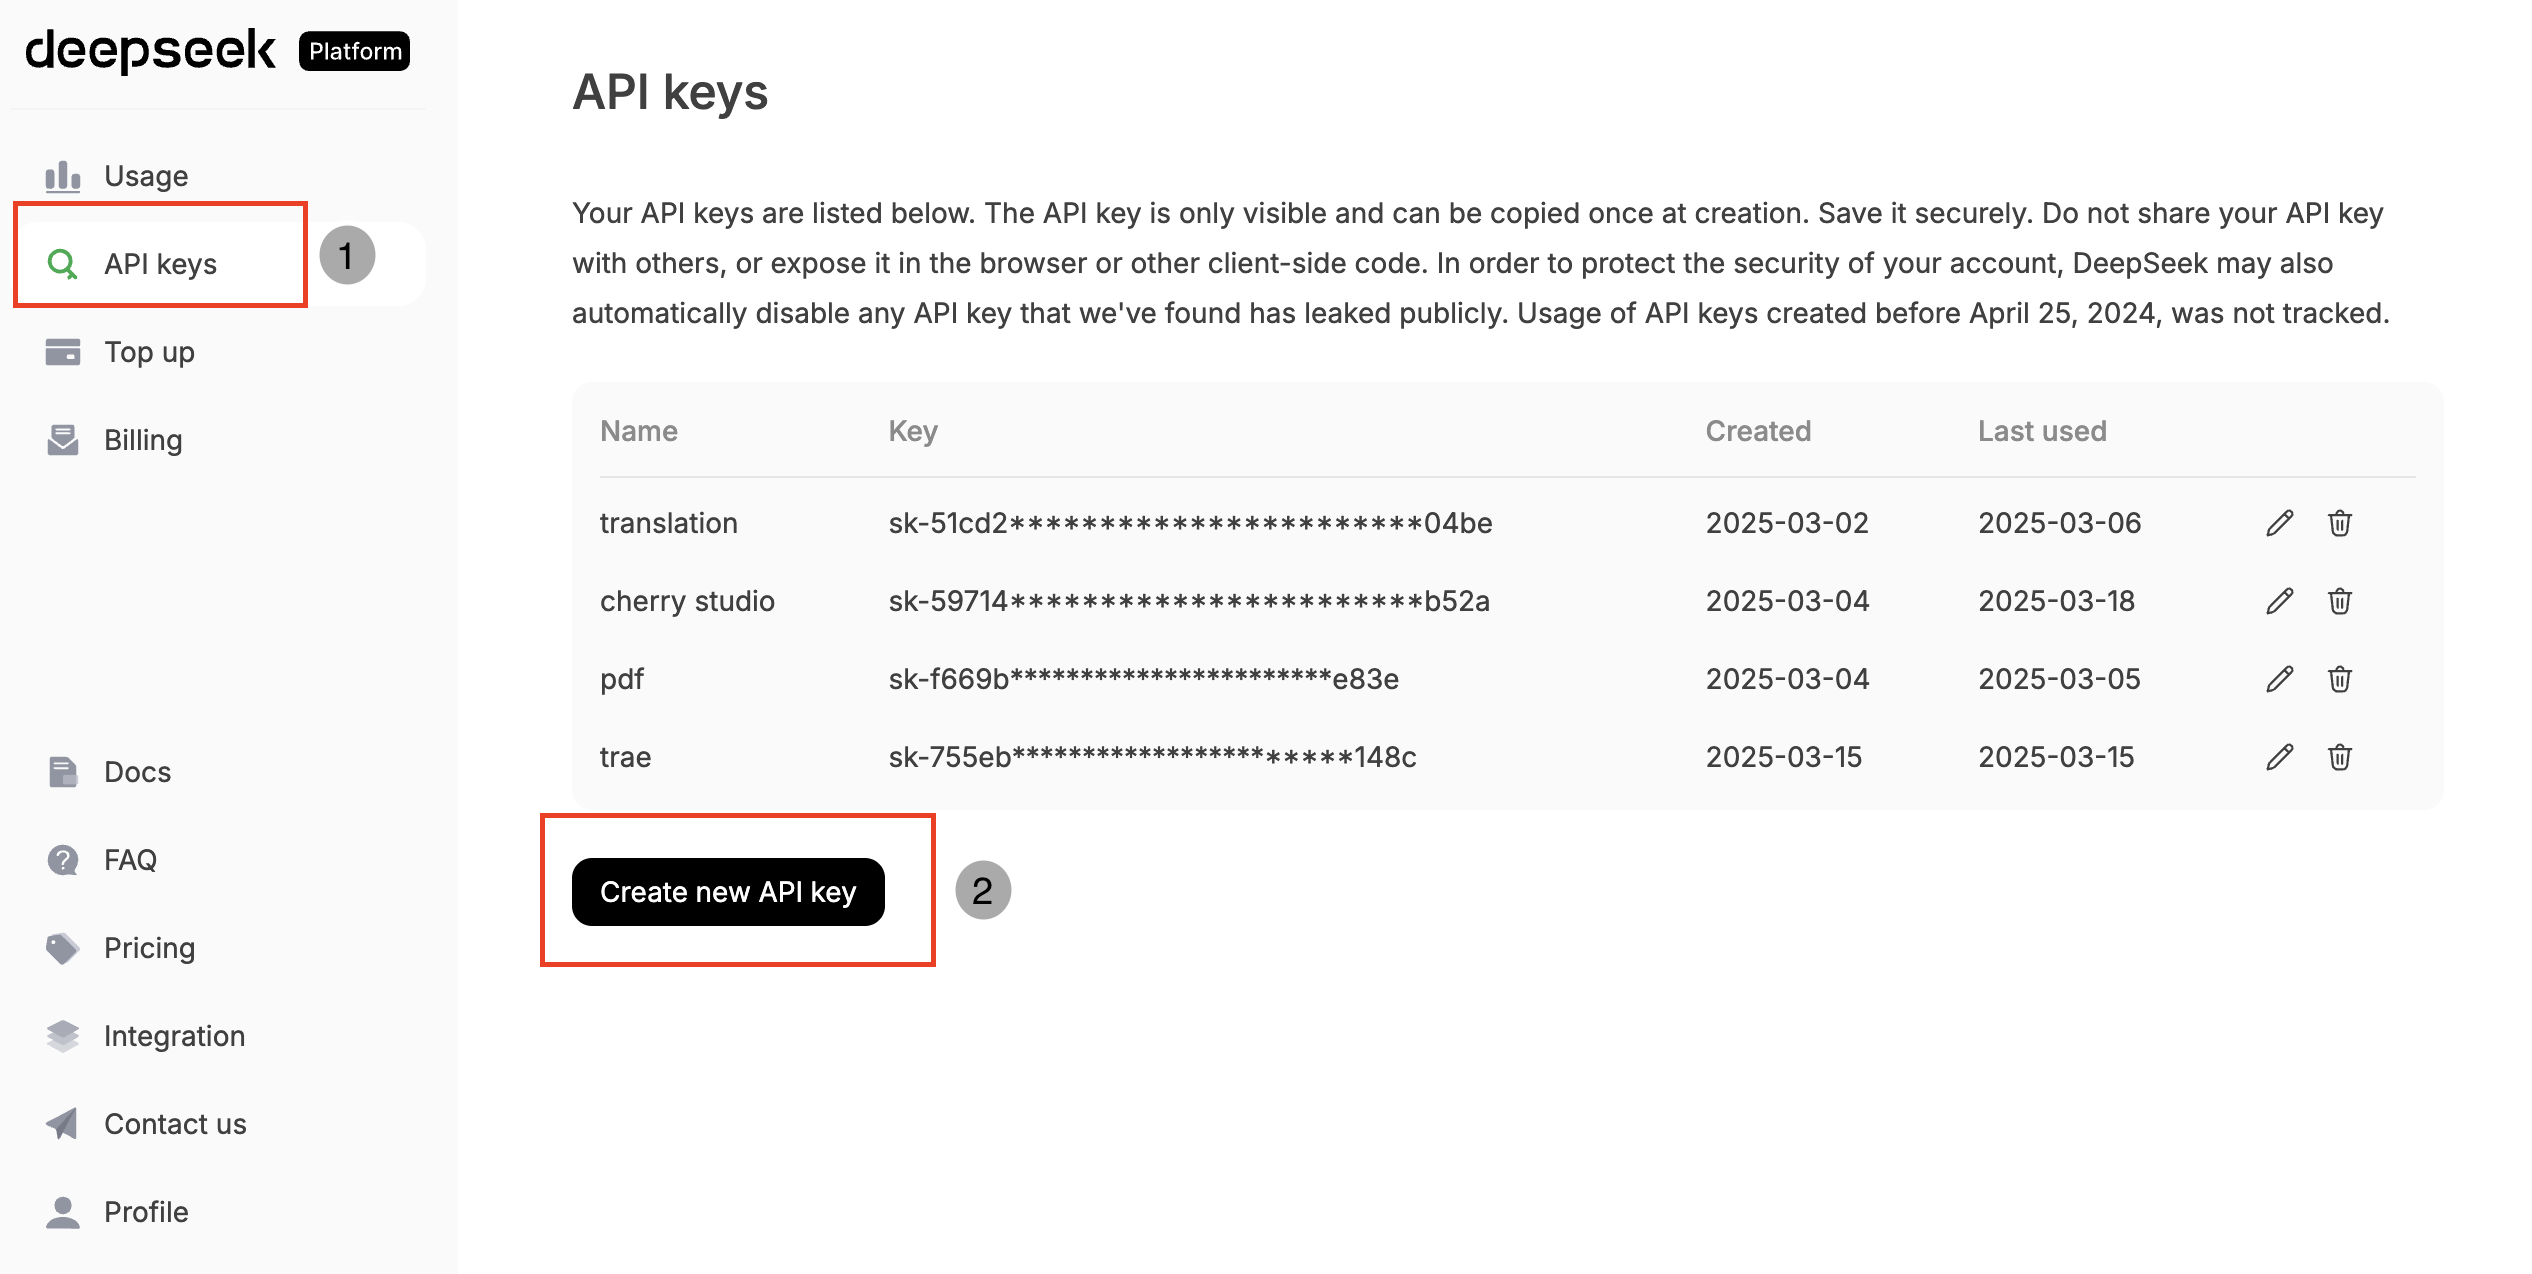
\includegraphics[width=1\linewidth]{figs/API2.png}
		\end{figure}
		
	\end{itemize}
\end{frame}

\begin{frame}{主流大语言模型API Key的获取}
	\begin{itemize}
		\item  \textbf{国外厂商:}通常需要通过境外信用卡支付,对网络条件有一定要求。
		\item[] 解决方案(仅作参考):
		\begin{enumerate}
			\item 使用虚拟信用卡\url{https://yeka.ai},优化网络环境。
			\item 使用代理服务商\url{https://openrouter.ai}
		\end{enumerate}
	\end{itemize}
\end{frame}

\begin{frame}{API参考定价 (2025-03-09)}
    \scriptsize
    \begin{table}[htbp]
        \centering
        \begin{tabular}{lll}
        \hline
        \textbf{机构} & \textbf{模型} & \textbf{输入/输出价格(美元/百万tokens)} \\
        \hline
        阿里 & Qwen-max & 1.6 / 6.4 \\
             & Qwen-plus & 0.4 / 1.2 \\
        \hline
        OpenAI & GPT-4o & 2.5 / 10 \\
               & GPT-4o-mini & 0.15 / 0.6 \\
               & o1 & 15 / 60 \\
        \hline
        谷歌 & Gemini 2.0 Flash & 0.1 / 0.4 \\
             & Gemini 2.0 Flash-Lite & 0.075 / 0.3 \\
             & Gemini 1.5 Flash & 0.075 / 0.3 \\
        \hline
        Anthropic & Claude 3.7 Sonnet & 3 / 15 \\
                  & Claude 3.5 Haiku & 0.8 / 4 \\
                  & Claude 3 Sonnet & 15 / 75 \\
        \hline
        深度求索 & deepseek-chat & 0.27 / 1.1 \\
                & deepseek-reasoner & 0.55 / 2.19 \\
        \hline
        月之暗面 & kimi-latest (8k–128k) & 1.62–8.1 / 1.62–8.1 \\
        \hline
        字节跳动 & Doubao-pro (4k-256k) & 0.1-0.675 / 0.27-1.215 \\
        \hline
        \end{tabular}
        \\[5pt]
        \begin{flushleft}
            \tiny
            \textbf{注意:}实际使用中,不同厂商有不同优惠政策,成本可能更低。\\
            \textbf{输入价格}:上传至模型的数据收费;
            \textbf{输出价格}:模型返回结果的数据收费。\\
            \textbf{tokens} 为模型处理文本的基本计量单位,通常一个汉字约等于 0.6 个 tokens,一个英文单词约等于 0.3 个 tokens。
            \end{flushleft}
        \end{table}
        
\end{frame}

\begin{frame}[fragile]{代码详细说明 (Python)}
    \scriptsize
\textbf{使用openai库:} 目前主流厂商的API调用都可以通过openai库实现,因此仅展示openai库的使用方法。

\begin{lstlisting}[language={Python}]
from openai import OpenAI  
client = OpenAI()  # 初始化OpenAI客户端,可填入API Key与url网址
prompt = "You are a helpful assistant"  # 系统角色提示
input_text = "What is the capital of France?"  # 用户输入问题
completion = client.chat.completions.create(
    model="gpt-4o",  # 指定模型
    messages=[ 
        {"role": "system","content": prompt},  # 系统角色消息
        {"role": "user","content": inquire1},  # 第一轮对话用户角色消息
        {"role": "assistant","content": output1} , #  AI返回消息
        {"role": "user","content": input_text}  # 第二轮对话输入信息
    ],
    temperature=1,  # 温度1为最高
    max_tokens=2048,  # 限制生成最大长度
    top_p=1,  # 采样策略1为全概率
    frequency_penalty=0,  # 禁用重复惩罚
    presence_penalty=0  # 禁用主题惩罚
)
print(completion.choices[0].message.content)  # 输出首个响应内容
#输出示例:The capital of France is Paris.
\end{lstlisting}
\end{frame}

\begin{frame}[fragile]{代码详细说明: 重要参数解析}
    \begin{itemize}
        \item \textbf{model}:指定模型版本,如 "gpt-4o"、"deepseek-chat"。
        \item \textbf{messages}:构建对话历史(系统、用户、助手)。
        \item \textbf{temperature}:控制随机性,数值越高生成越多样。
         \item \textbf{top\_p}:随机采样策略,作用与temperature相同。
        \item \textbf{max\_tokens}:限制返回文本的最大长度。
        \item \textbf{frequency\_penalty} \& \textbf{presence\_penalty}:调整重复率和新话题引入。
    \end{itemize}
    \medskip
    \textbf{建议:} 根据任务需求调整参数,如创意写作可提高temperature,事实查询则建议降低temperature,但是tempreature与top\_p不能同时修改。
\end{frame}

\begin{frame}[fragile]{API调用进阶2:多线程调用}
\small
    在实际应用中,为了提高API调用效率,可以采用多线程并发处理多个请求。多线程调用的优势包括:
    \begin{itemize}
        \item \textbf{提高响应速度} 
        \item \textbf{更高的处理量} 
    \end{itemize}
    具体代码示例,已保存在项目库中,可进一步查看。

    \textbf{注意:} 由于大部分平台都有访问流量上限,使用多线程时需要特别注意线程数量不能超过限制。
\end{frame}

\begin{frame}[fragile]{实际应用:使用大语言模型提取上海市历年经济增长目标}

	\begin{enumerate}
		\item 遍历文件夹,将政府工作报告文本、年份、城市名,整理成规范表格
		\item 选择合适模型,获取所需要模型的API Key
		\item 使用多线程方法,批量调用大语言模型处理文本
		\item 等待结果返回
	\end{enumerate}

\end{frame}

\begin{frame}[fragile]
	\begin{itemize}
		\item 最终结果:由于工作报告文本量较大,处理20个样本最终耗时2分钟,计费0.1元
		\item 处理结果展示
		\begin{figure}[htpb]
			\centering
			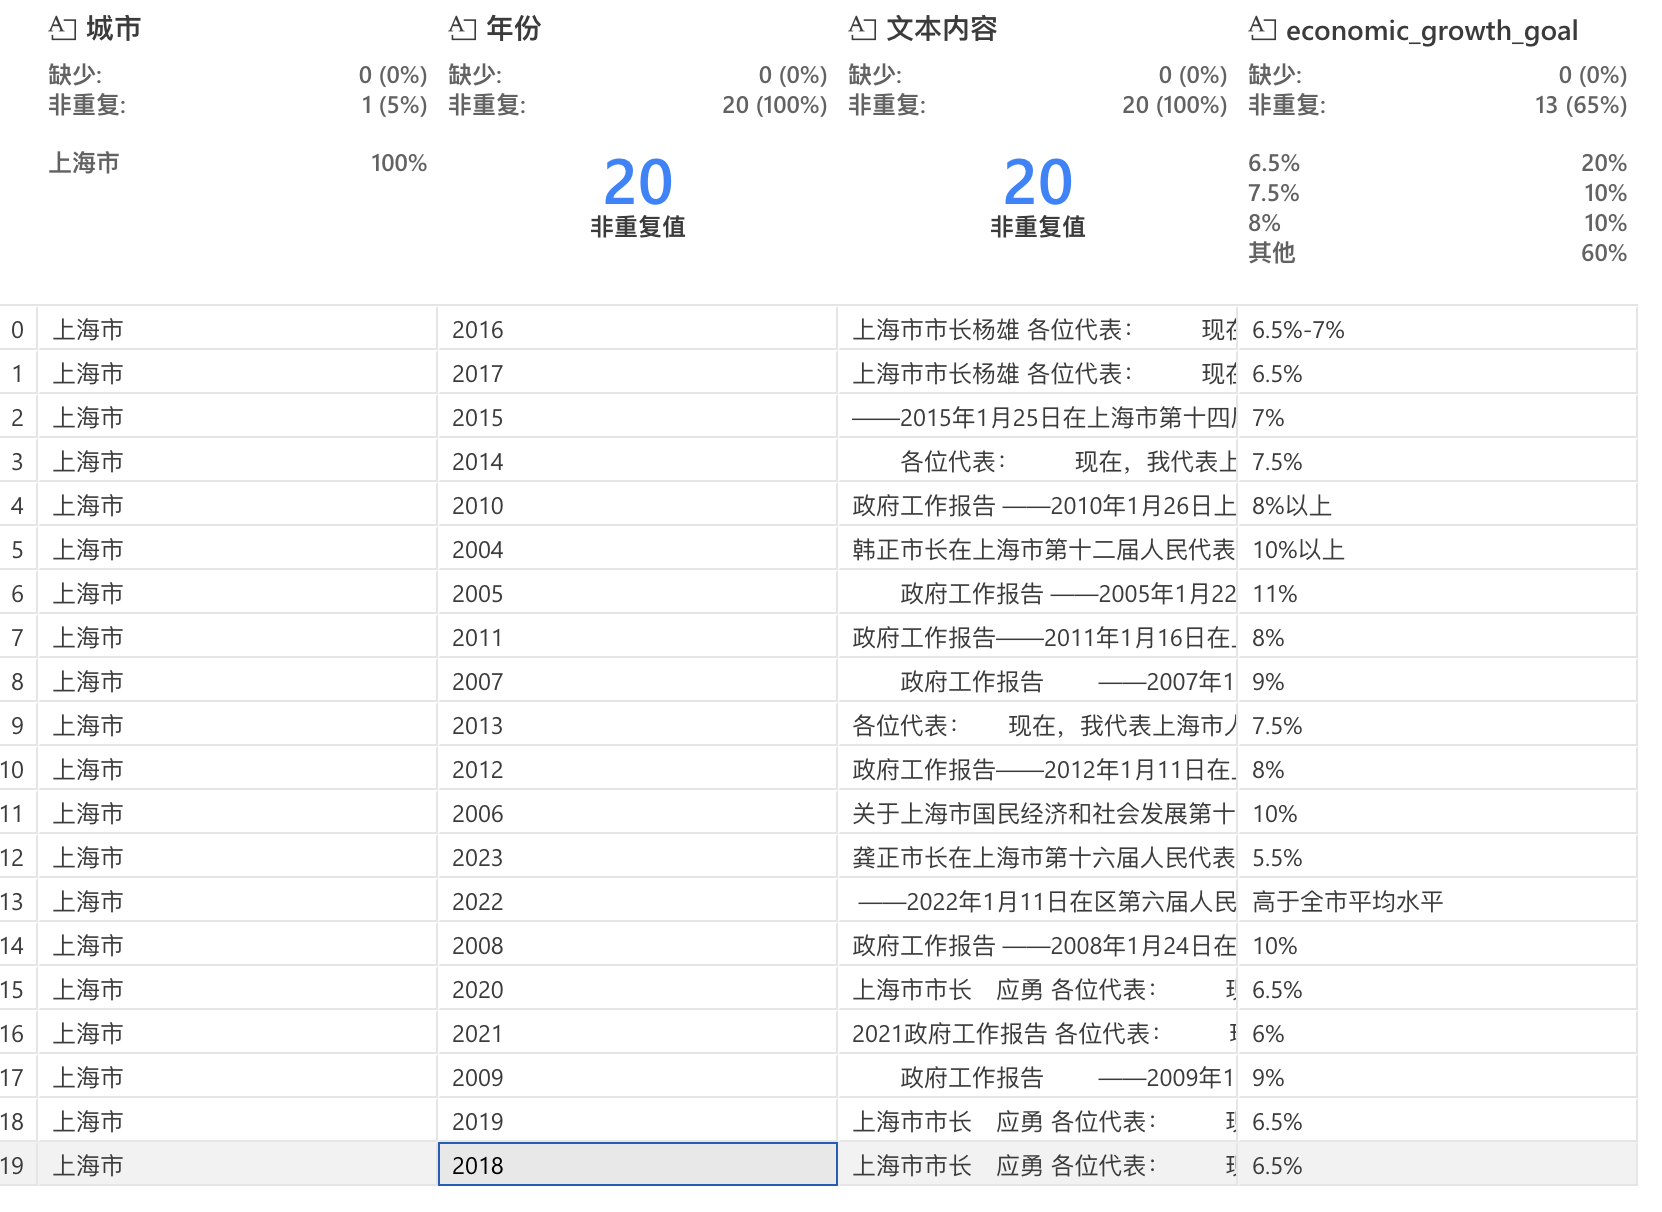
\includegraphics[width=0.8\linewidth]{figs/处理结果.png}
		\end{figure}
		\item 2022年工作报告原文:“2022年全区经济社会发展的主要预期目标是:地区生产总值增速高于全市平均水平,区级一般公共预算收入增长8\%”
	\end{itemize}
\end{frame}

%=================================================
\section{如何强化大语言模型在特定领域的理解力}
\begin{frame}[fragile] {引言}
	\begin{itemize}
		\item \textbf{可靠性}是学术研究的关键,在实际论文中使用大语言模型构造X、Y,仍有两个问题还需解决:
		\item \textbf{如何使大语言模型掌握处理特定文本数据的能力?}
		\item \textbf{如何证明大语言模型确实掌握了这个能力?}


\item \textbf{解决方案:}
	\begin{enumerate}
	\item 设计合理提示词(Prompt)
	\item 构造知识库(RAG)
	\item 对大语言模型进行微调(Fine-Tunning)
\end{enumerate}
	\end{itemize}
\end{frame}

%=================================================
\subsection{Prompt Engineering(提示词工程)}
\begin{frame}[fragile]{Prompt工程}
    \small
\begin{itemize}
  \item 	\textbf{什么是Prompt} 如果把大语言模型比作工人,Prompt就相当于指导工人的号令。
  \item \textbf{为什么还需要prompt?}虽然目前最先进大语言模型已内置思维链,使用时无需复杂提示,但经济学领域的任务多为文本分类和语义识别。此时,采用思维链模型成本较高且优势不明显,因此应选择效果好且经济的方案。
  \item \textbf{什么是好的prompt?} 好的prompt应具备以下特点:
   \begin{enumerate}
      \item 明确任务目标。
      \item 提供清晰的输入。
      \item 明确期望的输出格式。
      \item 提供思维链。
      \item 指令保证格式清晰
    \end{enumerate}
\end{itemize}
\textbf{小贴示:} 
\begin{itemize}
    \item 众多API平台都提供了prompt生成功能,可以先在对应平台生成prompt再进行修改。
\end{itemize}
\end{frame}

\begin{frame}[fragile]{Prompt示例}

       \begin{figure}[ht]
\flushleft
	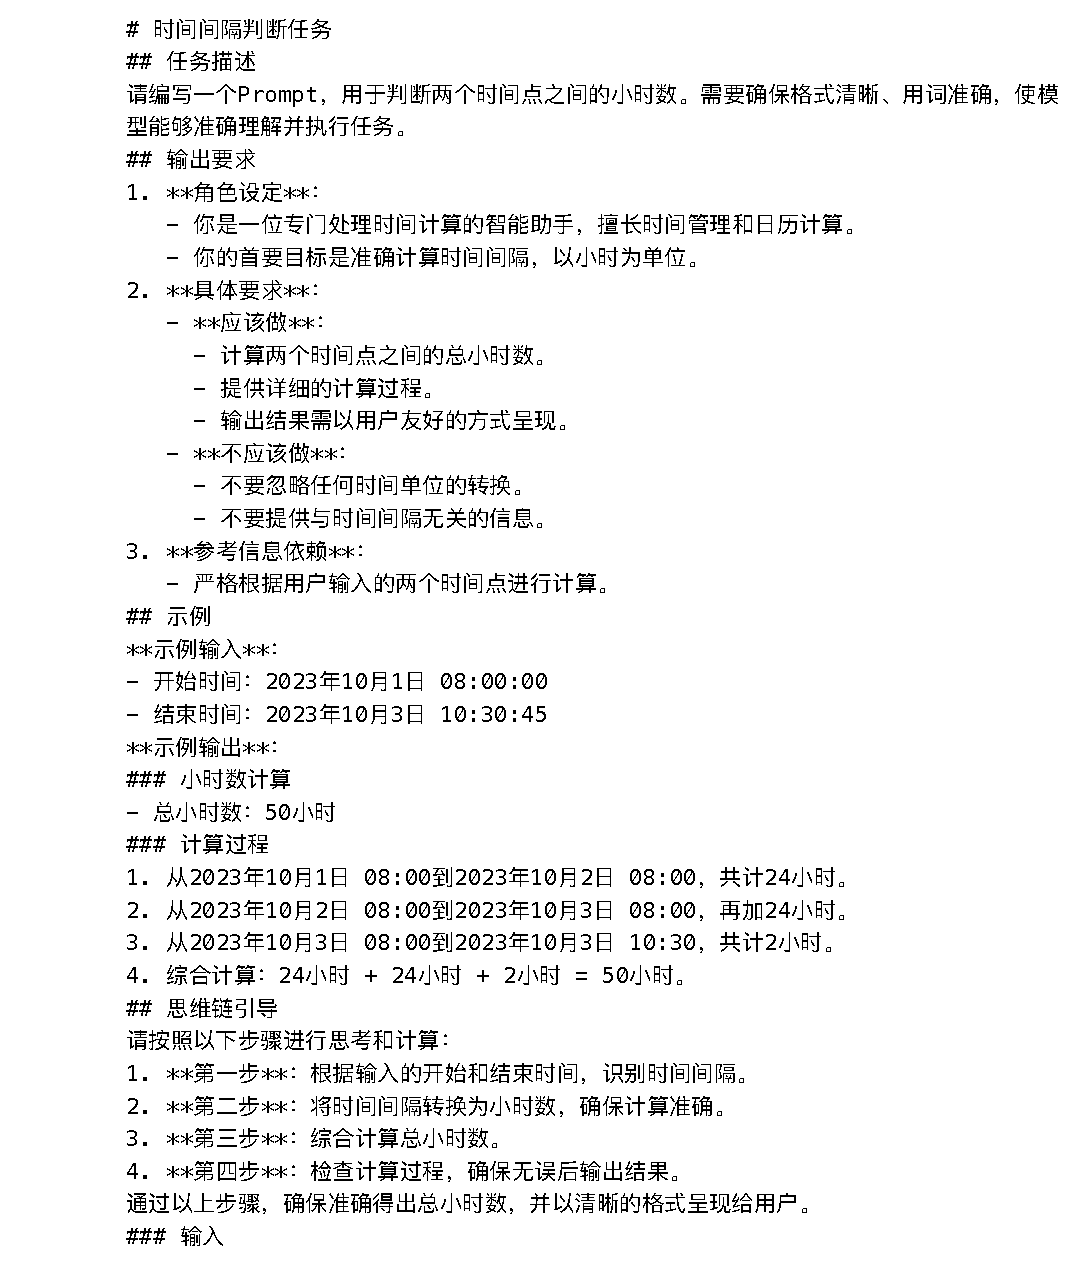
\includegraphics[height=0.85\textheight]{figs/prompt示例.pdf}
\end{figure}
\end{frame}

\subsection{RAG(检索增强生成)}
\begin{frame}[fragile]{构建知识库}
\small
\begin{itemize}
	
\item \textbf{什么是RAG} 如果把大语言模型比作工人,知识库就相当于指导工人如何工作的手册,可供其翻阅。

\item 目前主流API平台,如:阿里、coze,大多支持上传pdf、word、txt等格式的文档来构建知识库,在调用过程中,模型可从知识库中读取知识来提高回复质量。

\item 与直接使用大语言模型相比,RAG具有以下特点:
\begin{enumerate}
    \item \textbf{成本更低:} 只收取上传一次时的费用,后续不再收费
    \item \textbf{更高效:} 利用文档中的信息作为上下文,能提高生成回答的准确性和完整性
 \item \textbf{文本读取相对随机:} “工人”是否会读取知识库,会受到知识库多大影响无法准确衡量。因此,知识库并不适用于严肃的应用场景。
\end{enumerate}
\end {itemize}
\end{frame}

\begin{frame}[fragile]{知识库 vs 非知识库回答}
\small
\textbf{问题:} 简要概括什么是企业绿色发展?

\textbf{知识库:}由10篇关于企业绿色发展的论文组成。

\begin{table}[h]
\centering
\scriptsize
\begin{tabular}{|p{0.5cm}|p{4.5cm}|p{4.3cm}|}
\hline
\textbf{} & \textbf{使用知识库} & \textbf{不使用知识库} \\
\hline
回答 & 
企业绿色发展是指企业以绿色发展理念为指导,通过资源集约利用和环境友好为导向,以绿色创新为核心,实现生产全过程的绿色化,同时兼顾经济绩效和环境绩效,最终达到生态环境改善和经济社会高质量发展的目标。这一过程涉及环境绩效、经济绩效和绿色创新绩效三个方面。环境绩效表现为企业在绿色转型过程中为保护环境和治理污染所取得的成绩;经济绩效是企业通过资源分配与利用所获得的效益;绿色创新绩效则是企业通过绿色创新积蓄的技术驱动力 。
& 
企业绿色发展是指企业在生产经营过程中,通过采用环保技术、优化资源利用、减少污染排放、降低能源消耗等措施,实现经济效益与环境保护的双赢。其核心在于将可持续发展理念融入企业战略和日常运营中,推动经济增长与生态环境保护的协调统一。企业绿色发展不仅有助于减少对环境的负面影响,还能提升企业竞争力,满足社会对环保的期望,促进长期可持续发展。 \\
\hline
\end{tabular}
\end{table}

\textbf{分析:}同一个模型,引入知识库后,回答更倾向于目前学术研究的关注方向,与不使用知识库的回答有较大区别。

\end{frame}

\subsection{Fine-Tuning(微调)}
\begin{frame}[fragile]{通过微调强化特定领域能力}
\small
\begin{itemize}
	
	\item \textbf{什么是微调?}:如果把大语言模型比作工人,微调就相当于使用实现准备好的针对性教材(数据),以上课的方式,对大语言模型的思维模式进行改进,以适应新工作。
	\item \textbf{为什么要微调?}:通过微调一方面可以提升模型处理数据的能力,另一方面也可以验证模型处理数据的可靠度。
\end{itemize}
\textbf{微调步骤:}
\begin{enumerate}
    \item 准备并上传训练数据
    \item 训练新的微调模型
    \item 评估结果并根据需要返回步骤 1
    \item 使用微调模型
\end{enumerate}
\end{frame}

\begin{frame}[fragile]{如何准备微调数据:}

\begin{enumerate}
    \item \textbf{数据标注}:根据需要处理的目标任务,针对性的提供一系列回答的结果示例。
    \item \textbf{数据格式化}:将预处理后的数据转换为模型所需的格式。常见格式有 JSON、CSV 等。例如,在基于文本分类的微调中,由于要求回答相对单一,可以采用如下格式:
    \begin{verbatim}
{"prompt": "请你判断“今天股票又亏了三个点”
属于乐观还是悲观?", "completion": "悲观"}
    \end{verbatim}
    \item \textbf{数据扩增(可选)}:当可用数据量不足时,可考虑使用数据扩增技术,如同义句生成、数据混合或噪声注入等方法,增加数据多样性,提高模型鲁棒性(稳定性)。
\end{enumerate}

关于微调的具体介绍,已保存在项目库中,可进一步查看。
\end{frame}

\begin{frame}[fragile]{微调测试案例}
    \small
    \textbf{测试案例一:}\\[0.5em]
    \textbf{采购公告:}怒江州林业局森林防火地理信息指挥系统采购项目中标公示\\[1em]
    \begin{tabular}{llll}
    \toprule
    是否微调 & 是否需要prompt & 模型名称 & 分类结果 \\
    \midrule
    是 & 否 & ERNIE 4.0   & 两者 \\
    否 & 是 & ERNIE 4.0      & (未能识别任务) \\
    否 & 是 & GPT-4o            & 两者 \\
    否 & 是 & GPT-4o-mini       & 两者 \\
    \bottomrule
    \end{tabular}
  
    \textbf{结果发现:}\\[0.5em]
    微调后的 ERNIE 4.0 在识别准确性上大致接近于未经过微调的 GPT-4o-mini。\\
    后续查询相关论坛帖子,发现如果只是对文本进行分类处理,只要选择足够优秀的大语言模型,微调并不必要。
    \end{frame}
    


%=================================================
\section{在经济学领域应用的具体案例}
%=================================================
%%%%%%%%%%%%%%%%%%%%%%%%%%%%%%%%%%%%%%%%%%%%%%%%%%%%
% 案例一:大语言模型、文本情绪与金融市场
%%%%%%%%%%%%%%%%%%%%%%%%%%%%%%%%%%%%%%%%%%%%%%%%%%%%
\begin{frame}{案例一:大语言模型、文本情绪与金融市场(姜富伟等,2024)}
    \textbf{主要研究内容:}
    \begin{itemize}
      \item 构建中文金融大语言模型,用于预测金融市场情绪、资产价格回报等。
      \item 将结构化的市场数据(如股价、回报率)与非结构化文本数据(如财经新闻、公司公告)相结合,通过大模型更精准地刻画金融市场非理性情绪。
    \end{itemize}
    
    \textbf{核心技术方案:}
    \begin{itemize}
      \item 以 BERT/ERNIE 类深度学习模型为基础做预训练与微调。
      \item 引入市场回报标签,进行有监督的情绪分类或回归预测。
      \item 对比传统字典法,验证“大模型情绪”在极端市场状况下的预测优越性。
    \end{itemize}
    \end{frame}
    
    \begin{frame}{案例一:实现过程}
    \begin{itemize}
      \item \textbf{思路:} 
      \begin{itemize}
        \item 在通用预训练模型基础上,利用市场回报数据作为情绪标签进行有监督微调。
      \end{itemize}
      \item \textbf{具体流程:}
      \begin{enumerate}
        \item \textbf{选定预训练模型:}如 BERT、ERNIE、RoBERTa 等。
        \item \textbf{标注数据集:}以股票收益正负为情绪标签(0/1 分类),或多档位标签。
        \item \textbf{模型评估:}分类准确率、F1-score、在样本外的收益预测表现等。
        \item \textbf{模型部署:}调用API,将微调好的模型用于未来新闻文本情绪批量处理。
      \end{enumerate}
      \item \textbf{效果:}
      \begin{itemize}
        \item 明显优于传统字典法,捕捉到非线性、上下文关联和极端事件下情绪冲击。
      \end{itemize}
    \end{itemize}
    \end{frame}
    
    
    %%%%%%%%%%%%%%%%%%%%%%%%%%%%%%%%%%%%%%%%%%%%%%%%%%%%
    % 案例二:企业数字化转型的测度难题
    %%%%%%%%%%%%%%%%%%%%%%%%%%%%%%%%%%%%%%%%%%%%%%%%%%%%
    \begin{frame}{案例二:企业数字化转型的测度难题(金星烨等,2024)}
    \textbf{主要研究内容:}
    \begin{itemize}
      \item 提出用大语言模型识别上市公司年报中是否真实应用数字技术(如 AI、大数据、云计算等),从而构建更准确的数字化转型指标。
      \item 解决传统词典法关键词遗漏和误判等问题,进而研究数字化转型对企业绩效的影响差异。
    \end{itemize}
    
    \textbf{核心技术方案:}
    \begin{itemize}
      \item 采用大语言模型(如 ERNIE)对年报句子逐句判定是否涉及数字技术以及数字技术类型。
      \item 与人工标注结合,“进一步预训练”+ 微调,在构造新指标时更加完备且准确度更高。
    \end{itemize}
    \end{frame}
    
    \begin{frame}{案例二:实现过程}
    \begin{itemize}
      \item \textbf{数据标注:}
      \begin{itemize}
        \item 提前选定一个人工标注数据集(部分年报句子),区分是否真实采用数字技术。
      \end{itemize}
      \item \textbf{微调过程:}
      \begin{enumerate}
        \item 在已有的中文模型(如 ERNIE)上进行“进一步预训练”(further pretraining),让模型适应企业年报用语。
        \item 基于标注数据进行分类微调:句子 $\rightarrow$ 是否包含“真实使用数字技术”。
        \item 最终模型在测试集上评估指标,如 Accuracy、Precision、Recall、F1-score 等。
      \end{enumerate}
      \item \textbf{效果:}
      \begin{itemize}
        \item 相较于关键词检索法,显著降低误判(谈技术却未实际应用)与漏判(实际应用技术却关键词缺失)的概率。
      \end{itemize}
    \end{itemize}
    \end{frame}


%=================================================
\section{基于大语言模型的开源项目分享}
%=================================================
\subsection{Chatbox \& CherryStudio}
\begin{frame}{Chatbox \& CherryStudio:通过API实现各平台大语言模型集成}
  \begin{itemize}
    \item \textbf{概述:} 基于API调用机制,可以通过上传API的形式,实现各平台大语言模型的集成。
    \item \textbf{优势:} 将API调用可视化实现类似于网页的功能;热门模型如deepseek网页端经常卡顿,但是使用API调用则不会。
  \end{itemize}
\end{frame}

\subsection{PDF2zh}
\begin{frame}{PDF2zh:将大语言模型引入pdf文献翻译}
  \begin{itemize}
    \item 已有翻译引擎仅限于机翻,少部分可以使用AI的翻译软件并不能提供全文翻译
    \item 此项目可以将PDF全文翻译为中文,并保留排版格式,方便阅读。
    \item 由于项目自身基于命令行,且其可视化窗口配置较为复杂。基于此项目开发了可视化项目,也可供参考:\url{https://github.com/luzhiyu-econ/PDF-Translator}
  \end{itemize}
\end{frame}

\subsection{Ollama}
\begin{frame}{Ollama: 本地开源大模型部署}
  \begin{itemize}
    \item 依据本地计算机算力,主要受电脑显卡显存于电脑内存限制,可以在本地部署不同的大语言模型模型。并开放API供用户调用。
    \item 通过本地调用模型一方面节省了API费用;另一方面,也规避了后续官方模型调整,原实验结果不可复现的局面。
  \end{itemize}
\end{frame}

\subsection{其他}
\begin{frame}{其他}
  \begin{itemize}
    \item Cursor,Trae: AI powered IDE
    \item 将AI功能集成到IDE中,可以实现代码生成、代码解释、代码调试等功能。
  \end{itemize}
\end{frame}

%------------------------------------------------
\begin{frame}{References}
  \footnotesize
  \begin{thebibliography}{10}

  \bibitem{dell2023}
    Dell, M. (2023).
    \newblock Deep Learning for Economists.
    \newblock \emph{Journal of Economic Literature}.

  \bibitem{korinek2023}
    Korinek, A. (2023).
    \newblock Generative AI for Economic Research: Use Cases and Implications for Economists.
    \newblock \emph{Journal of Economic Literature}.

  \bibitem{hong2024}
    Hong, Y. \& Wang, S. (2024).
    \newblock ChatGPT 与大模型将对经济学研究范式产生什么影响?
    \newblock \emph{计量经济学报}.

  \end{thebibliography}
\end{frame}

\end{document}